\documentclass{article}
\usepackage{titling}
\usepackage{lipsum}
\usepackage{amsmath}
\usepackage{listings}
\usepackage{graphicx}
\usepackage{subcaption}
\usepackage{pgfplots}
\usepackage[margin=1in]{geometry}
\usepgfplotslibrary{statistics}



\begin{document}
\noindent

\begin{center}
    \vspace*{0.3\textheight}
    {\fontsize{80}{18}\textbf{Math 343 - Final Project}}\\
    \vspace{6pt} % add 6pt of vertical space
    \rule{0.87\linewidth}{1pt}\\ % 80% of the width, thickness: 1pt
    \vspace{12pt} % add 6pt of vertical space
    \LARGE\textbf{Word Frequency Counting Optimization in Java}\\
    
    \vspace{12pt}
    \Large\textbf{Preston Duffield} \\
    \Large duffiep@wwu.edu \\
    \Large Western Washington University \\
    \today
    % April 18, 2023
    \vspace{24pt}
\end{center}

\clearpage
\section*{Introduction}



\section*{Analysis of Data}
Statisical analysis was performed with Minitab.
The objective of the analysis was to determine what factors were
significant in affecting the runtime in seconds of the computer program.

\subsection*{Anova Analysis}
\begin{figure}[h]
  \centering
  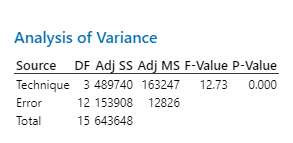
\includegraphics[width=0.5\textwidth]{./images/2_a.png}
  \caption{ANOVA table from Minitab.}
  \label{fig:2_a}
\end{figure}


\section*{Residual Analysis}
\section*{Conclusion}

\clearpage
\appendix
\section*{Appendix}
\subsection*{Java Code}
\begin{lstlisting}[language=Java, 
  basicstyle=\ttfamily\scriptsize, 
  numbers=none, 
  frame=single,
  showspaces=false,
  caption={Source Code for the WordFrequencyCounter.java file.}]
  import java.io.*;
  import java.nio.file.*;
  import java.util.*;
  
  public class WordFrequencyCounter {
    private static long startTime;
  
    public static void main(String[] args) throws IOException {
      if (args.length != 4) {
        System.err.println(
            "Usage: WordFrequencyCounter <buffer size> <algorithm> <input file> <quiet flag>");
        System.exit(1);
      }
  
      int bufferSize = Integer.parseInt(args[0]);
      String algorithm = args[1];
      Path inputFilePath = Paths.get(args[2]);
      boolean isQuiet = Boolean.parseBoolean(args[3]);
  
      if (!Files.exists(inputFilePath)) {
        System.err.println("The input file does not exist.");
        System.exit(2);
      }
  
      startTime = System.currentTimeMillis();
  
      switch (algorithm.toLowerCase()) {
        case "hashmap":
          hashMapApproach(inputFilePath, bufferSize, isQuiet);
          break;
        case "sorting":
          sortingApproach(inputFilePath, bufferSize, isQuiet);
          break;
        default:
          System.err.println("Invalid algorithm type. It should be 'hashmap' or 'sorting'.");
          System.exit(3);
      }
  
      long endTime = System.currentTimeMillis();
      double totalTimeInSeconds = (endTime - startTime) / 1000.0;
      System.out.printf("Total time: %.4f seconds.%n", totalTimeInSeconds);
    }
  
    private static void
        hashMapApproach(Path filePath, int bufferSize, boolean isQuiet) throws IOException {
      try (BufferedReader reader = new BufferedReader(new FileReader(filePath.toFile()), bufferSize)) {
        HashMap<String, Integer> wordCount = new HashMap<>();
        String line;
  
        while ((line = reader.readLine()) != null) {
          String[] words = line.split("\\s+");
          for (String word : words) {
            wordCount.put(word, wordCount.getOrDefault(word, 0) + 1);
          }
        }
  
        if (!isQuiet) {
          for (Map.Entry<String, Integer> entry : wordCount.entrySet()) {
            System.out.println(entry.getKey() + ": " + entry.getValue());
          }
        }
      }
    }
  
    private static void
        sortingApproach(Path filePath, int bufferSize, boolean isQuiet) throws IOException {
      try (BufferedReader reader = new BufferedReader(new FileReader(filePath.toFile()), bufferSize)) {
        ArrayList<String> wordList = new ArrayList<>();
        String line;
  
        while ((line = reader.readLine()) != null) {
          String[] words = line.split("\\s+");
          wordList.addAll(Arrays.asList(words));
        }
  
        Collections.sort(wordList);
  
        if (!isQuiet) {
          int count = 1;
          for (int i = 1; i < wordList.size(); i++) {
            if (wordList.get(i).equals(wordList.get(i - 1))) {
              count++;
            } else {
              System.out.println(wordList.get(i - 1) + ": " + count);
              count = 1;
            }
          }
  
          // Print the last word in the list and its count
          System.out.println(wordList.get(wordList.size() - 1) + ": " + count);
        }
      }
    }
  }  
\end{lstlisting}

\clearpage
\subsection*{Python Code}
\begin{lstlisting}[language=Python, 
  basicstyle=\ttfamily\scriptsize, 
  numbers=none, 
  frame=single,
  showspaces=false,
  caption={Source Code for the run\_java\_experiments.py file}]
  import subprocess
  import csv
  import sys
  from tqdm import tqdm
  
  def main(replicants):
      # Define the mapping of parameters
      parameters = {
          'Buffer Size': {-1: '16', 1: '4096'},
          'Algorithm Type': {-1: 'sorting', 1: 'hashmap'},
          'Input File': {-1: 'bible.txt', 1: 'pride_and_prejudice.txt'}
      }
  
      # Define the combinations of parameters to run
      combinations = [
          [-1, -1, -1],
          [1, -1, -1],
          [-1, 1, -1],
          [1, 1, -1],
          [-1, -1, 1],
          [1, -1, 1],
          [-1, 1, 1],
          [1, 1, 1]
      ]
  
      # Prepare the CSV file
      with open('results.csv', 'w', newline='') as csvfile:
          fieldnames = ['Buffer Size', 'Algorithm Type', 'Input File', 'Seconds']
          writer = csv.DictWriter(csvfile, fieldnames=fieldnames)
  
          writer.writeheader()
  
          total = len(combinations) * replicants
          pbar = tqdm(total=total, ncols=120)
  
          # For each combination of parameters...
          for combination in combinations:
              # Repeat the experiment the desired number of times
              for i in range(replicants):
                  # Prepare the arguments for the Java program
                  args = ['java', 'WordFrequencyCounter.java']
                  args += [parameters[fieldnames[i]][combination[i]] for i in range(len(combination))]
                  args.append('true')
  
                  # Run the Java program and capture the output
                  result = subprocess.run(args, capture_output=True, text=True)
  
                  # Extract the time value from the output
                  time = float(result.stdout.split()[-2])
  
                  # Write the result to the CSV file
                  writer.writerow({
                      'Buffer Size': combination[0],
                      'Algorithm Type': combination[1],
                      'Input File': combination[2],
                      'Seconds': time
                  })
  
                  pbar.set_description(
                    f"Running {i+1}/{replicants} replicants for combination {combination}")
                  pbar.update()
          pbar.close()
  
  if __name__ == "__main__":
      main(int(sys.argv[1]))  
\end{lstlisting}

% Ideas
% Experimental Design Cube

\end{document}
